
%%%%%%%%%%%%%%%%%%%%%%% file typeinst.tex %%%%%%%%%%%%%%%%%%%%%%%%%
%
% This is the LaTeX source for the instructions to authors using
% the LaTeX document class 'llncs.cls' for contributions to
% the Lecture Notes in Computer Sciences series.
% http://www.springer.com/lncs       Springer Heidelberg 2006/05/04
%
% It may be used as a template for your own input - copy it
% to a new file with a new name and use it as the basis
% for your article.
%
% NB: the document class 'llncs' has its own and detailed documentation, see
% ftp://ftp.springer.de/data/pubftp/pub/tex/latex/llncs/latex2e/llncsdoc.pdf
%
%%%%%%%%%%%%%%%%%%%%%%%%%%%%%%%%%%%%%%%%%%%%%%%%%%%%%%%%%%%%%%%%%%%


\documentclass[runningheads,a4]{llncs}
\usepackage[dvipdfmx]{graphicx}
\usepackage{tikz}
\usetikzlibrary{automata}
\usetikzlibrary{arrows}
\usetikzlibrary{decorations.markings}

\usetikzlibrary{lindenmayersystems}
\bibliographystyle{junsrt}

\usepackage{url}
\urldef{\mailsa}\path|{alfred.hofmann, ursula.barth, ingrid.haas, frank.holzwarth,|
\urldef{\mailsb}\path|anna.kramer, leonie.kunz, christine.reiss, nicole.sator,|
\urldef{\mailsc}\path|erika.siebert-cole, peter.strasser, lncs}@springer.com|
\newcommand{\keywords}[1]{\par\addvspace\baselineskip
\noindent\keywordname\enspace\ignorespaces#1}

\begin{document}
\section{Heighway dragon}

The Heighway dragon is one of fractals.
It can be described by a binary sequence that is called ``paperfolding sequence" \cite{automatic}.

\subsection{Paperfolding sequence}
The paperfolding sequence is named after the following operation to generate it.
First, take a piece of paper and fold it in half lengthwise, then fold the result in half again, and so on.
Next, unfold the paper.
The resulting sequence $(P_i)_{i\geq0}$ of ``hills" (1) and ``valleys" (0) is a paperfolding sequence.
For example,  after one fold, we get the pattern in Figure~\ref{fig:dragon} (Left).
After two folds and ten folds, we get the respective patterns in Figure~\ref{fig:dragon} (Center) and (Right).

\begin{figure}[h]
\begin{minipage}[b]{0.3\hsize}
\centering
\scalebox{0.4}{
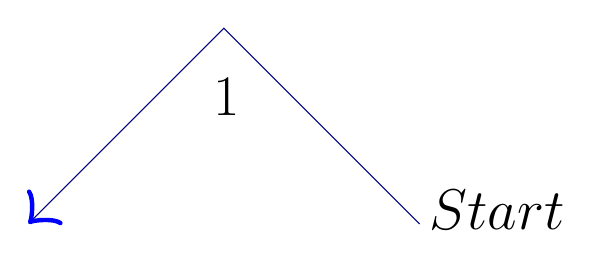
\begin{tikzpicture}
  \draw[blue!50!black,rotate=135,l-system={rule set={X->X+YF,Y->FX-Y},
  step=100pt,angle=90,axiom=FX,order=1},decoration={markings,mark=at position 1 with {\arrow[scale=5,blue]{>}}},
    postaction={decorate},
    shorten >=0.4pt] l-system;
  \coordinate (v) at (150:2.5) node at (v) [above left] {\huge$1$};	
  \node(st) at (10:1) {\huge$Start$};
\end{tikzpicture}
}
\end{minipage}
\begin{minipage}[b]{0.3\hsize}
\centering
\scalebox{0.3}{
\begin{tikzpicture}
  \draw[blue!50!black,rotate=135,l-system={rule set={X->X+YF,Y->FX-Y},
  step=100pt,angle=90,axiom=FX,order=2},
    decoration={markings,mark=at position 1 with {\arrow[scale=6,blue]{>}}},
    postaction={decorate},
    shorten >=0.4pt
    ] l-system;
  \coordinate (v) at (150:2.5) node at (v) [above left] {\huge$1$};	
  \coordinate (v) at (180:3.5) node at (v) [above left] {\huge$1$};
  \coordinate (v) at (225:3) node at (v) [above left] {\huge$0$};
  \node(st) at (10:1) {\huge$Start$};
\end{tikzpicture}
}
\end{minipage}
\begin{minipage}[b]{0.3\hsize}
\centering
\scalebox{0.015}{

\begin{tikzpicture}
  \draw[blue!50!black,rotate=135,l-system={rule set={X->X+YF,Y->FX-Y},
  step=100pt,angle=90,axiom=FX,order=10},-triangle 90] l-system;
\end{tikzpicture}
}
\end{minipage}
\caption{(Left) Heighway Dragon: One Fold. (Center) Heighway Dragon: Two Folds. (Right) Paperfolding Sequence: Ten Folds \cite{automatic}.}
\label{fig:dragon}
\end{figure}
The paperfolding sequence is a sequence that can be generated by the deterministic finite automaton with output (DFAO) in Figure~\ref{fig:pdfao} (automatic sequences).
Each state of a DFAO is assigned with a letter of an alphabet as an output.
Let ``n" be index of $P$ and, $n$ is non-negative integer.
We compute $P_n$ by feeding the DAFO with the base-2 representation of n, starting with least significant bit, and then applying an output alphabet of the last state reached.
Here are the first few terms of the limiting sequence.
\begin{eqnarray*}
n &=&\;0\; 1\;2\;3\;4\;5\;6\;7\;8 \ldots \\
P_n &=&\;1\; 1\;0\;1\;1\;0\;0\;1\;1 \ldots
\end{eqnarray*}

$P_n$ describes the Heighway Dragon as shown the exemplification in Figure~\ref{fig:dragon}.
For example, let ``0" of $P_n$ be ``right", and let ``1" of $P_n$ be ``left."
First, draw a line.
Next, $P_i$ is ``1", so turn left, and draw the line, then the pattern in Figure~\ref{fig:dragon} (Center) is obtained.
$P_2$ is also 1, so turn left, and draw a line.
$P_3$ is 0, so turn right, and draw a line, then the pattern in Figure~\ref{fig:dragon} is obtained.
We can elongate Heighway Dragon by repeating these process.
\begin{figure}[h]
  	\centering
	\scalebox{1}{
	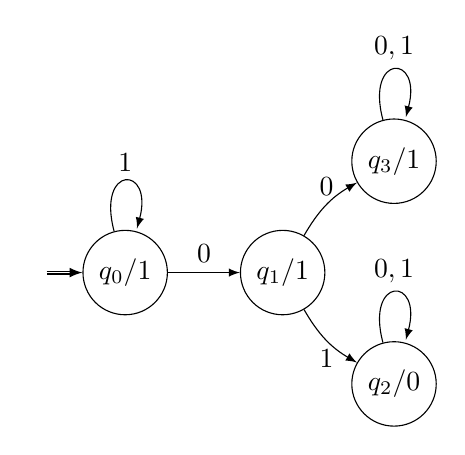
\begin{tikzpicture}[>=latex, node distance=2cm, initial text=, bend angle=15]
		 \tikzstyle{every initial by arrow} = [->, double];

		 \node [state, initial] (q_0)                        {$q_0/1$};
		 \node [state]                     (q_1) [right of = q_0]  {$q_1/1$};
		 \node [state]                     (q_2) [below right of = q_1] {$q_2/0$};
		 \node [state]                     (q_3) [above right of = q_1] {$q_3/1$};


 		\path [->] (q_0) edge [right] node [above]              {$0$}                 (q_1)
         		         edge [loop above] node [above]             {$1$}               ()
         			   (q_1) edge [bend left] node [above]             {$0$}                 (q_3)
         		         edge [bend right] node [below]             {$1$}              (q_2)
         			   (q_2)  edge [loop above] node [above]             {$0,1$}               ()
         			   (q_3)  edge [loop above] node [above]             {$0,1$}               ();
	\end{tikzpicture}
	}
\caption{DFAO for Paper folding sequence\cite{automatic}}
\label{fig:pdfao}
\end{figure}

\bibliography{reference}

\end{document}